%%%%%%%%%%%%%%%%%%%%%%%%
%%%%%%%%%%%%%%%%%%%%%%%%
%%%%%%%%%%%%%%%%%%%%%%%%
%%%%%%%%%%%%%%%%%%%%%%%%
%\subsection{Generalizing semistructured data integration}


%\subsubsection{Integrating graphs from semistructured sources with different associated schemas}

\label{sss:gdi}
After introducing the graphs as data structures on which we mined the correspondences for the alignment, we now want to generalize the data integration approach for semistructured data and choose to integrate them into  graphs. This time we will not integrate semistructured data using merged schema between the two sources as in Section \vref{sec:SDIIMRIACR}, but we will use a graph of choice as a target schema, thus resembling more what it has been outlined for $\qtransl$ in the LAV/GAV\index{data integration!local as a view}\index{data integration!global as a view} scenario. 

In order to simplify the more general problem, we will use as input  JSON (semistructured) data representing graphs using two different kinds of schemas. We use some notation that was already introduced during the formalization of schema correspondences and data modelling (Section \vref{sec:datamodelling}). In particular, we will start to analyse the data alignment applied to data provided with different non-GSM representation, both as inputs and outputs.


\begin{figure}[!t]
	\centering
	\begin{minipage}[!t]{0.8\textwidth}
		\centering
		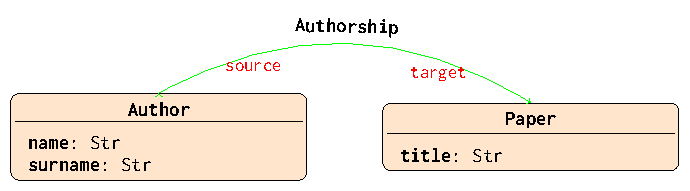
\includegraphics{fig/04model/06schema}
		\subcaption{Property graph representation.}
		\label{fig:schemawithsemantics}
	\end{minipage}
	
	\begin{minipage}[!t]{0.5\textwidth}
		\centering
		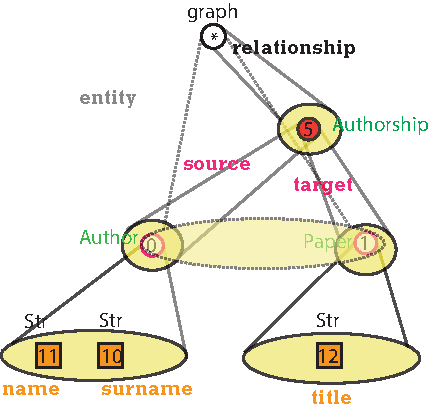
\includegraphics{fig/04model/01NestedToMatch.pdf}
		\subcaption{Nested graph representation.}
		\label{subfig:nestedhubforbiblio}
	\end{minipage}
	
	\caption{Representation of the hub schema providing the final desired representation of the JSON files after the alignment phase.}
\end{figure}
\lstdefinelanguage{theoryjson}
{
  % list of keywords
  morekeywords={
graph,nodes,id,label,metadata,data,meta,name,surname,title,source,destination,source,target,edges,fullname,graphs
  },
  sensitive=false, % keywords are not case-sensitive
  morecomment=[l]{//}, % l is for line comment
  morecomment=[s]{/*}{*/}, % s is for start and end delimiter
  morestring=[b]" % defines that strings are enclosed in double quotes
}

\begin{figure}[!p]
\centering
\lstinputlisting[language=Java,basicstyle=\ttfamily\small]{fig/04model/jsongraphspecif.json}
\caption{JSON representation $g$ of the graph presented in Figure \ref{fig:inputbibex} using the JSON Graph Format. {\url{http://jsongraphformat.info/}}}
\label{fig:jsongraphformat}
\end{figure}


\begin{figure}[!hpt]
\centering
\begin{minipage}[!t]{0.8\textwidth}
\centering
\lstinputlisting[language=Java,basicstyle=\ttfamily\small]{fig/04model/GRADOOPvertices.json}
\subcaption{Vertex representation, $v'$. Instead of representing both field ``name'' and ``surname, in this case we provide a ``fullname'' field for data integration explanatory reasons.}
\label{fig:gravertex}
\end{minipage}
\begin{minipage}[!t]{0.7\textwidth}
\centering
\lstinputlisting[language=Java,basicstyle=\ttfamily\small]{fig/04model/GRADOOPedges.json}
\subcaption{Edge representation, $e'$. The original tag ``target'' is here represented with the name ``destination'' for data integration explanatory reasons.}
\label{fig:graedge}
\end{minipage}
\caption{JSON representation $g'=(v',e')$ of the graph presented in Figure \ref{fig:inputbibex} using the GRADOOP JSON format  {\url{http://gradoop.org/}}, where vertices and edes are represented in different files.}
\label{fig:JSONGradoop}
\end{figure}

\begin{figure}[!p]
	\begin{minipage}[t]{\textwidth}
		\begin{lstlisting}[language=theoryjson,basicstyle=\ttfamily\small]
{ graph: { nodes: [({ id: Str,
                      label: Str,
                      metadata: { name: Str, surname: Str} + 
                                { title: Str }
		            })*],
		  edges: [({ id: Str,
		             label: Str,
		             source: Str,
		             target: Str,
		             metadata: {}
		           })*],
		}
}
		\end{lstlisting}
		\subcaption{Schema $\alpha(g)$ associated to the $g$ representation in Figure \ref{fig:jsongraphformat}}
		\label{fig:ajsongraphformat}
	\end{minipage}
	
	\begin{minipage}[t]{\textwidth}
		\begin{lstlisting}[language=theoryjson,basicstyle=\ttfamily\small]
[{ id: Str,
   data: { fullname: Str} + { title: Str},
   meta: { label: Str,
           graphs: [Str*]
		 }
}*]
		\end{lstlisting}
		\subcaption{Schema $\alpha(v')$ associated to the $v'$ representation in Figure \ref{fig:gravertex}}
		\label{fig:agravertex}
	\end{minipage}
	
	\begin{minipage}[t]{\textwidth}
		\begin{lstlisting}[language=theoryjson,basicstyle=\ttfamily\small]
[{ id: Str,
   data: {},
   source: Str,
   destination: Str,
   meta: { label: Str,
           graphs: [Str*]
		 }
 }*]
		\end{lstlisting}
		\subcaption{Schema $\alpha(e')$ associated to the $e'$ representation in Figure \ref{fig:graedge}}
		\label{fig:agraedge}
	\end{minipage}
	\caption{Extracting the schema associated to the JSON files representing some graphs. The same syntax of \cite{BaaziziLCGS17} is adopted.}
	\label{fig:ajsongraphrepr}
\end{figure}



\begin{example}[label=ex:examplegraphdata]
Suppose to have two bibliographic networks represented as bipartite graphs in JSON files using different schemas (see Example \vref{ex:bigraphbibnet}): we now want to integrate them into one final single graph. %Such bibliographic networks are exported using two JSON files using different formats. An example of 
Such formats are provided in Figure \ref{fig:jsongraphformat} ($g$ for short) and Figure \ref{fig:JSONGradoop} ($g'$ for short). %From two different JSON files we can always extract a schema using an automated process described in  \cite{BaaziziLCGS17}. 
Their respective schemas $\alpha(g)$ and $\alpha(g')$ are  provided in Figure \ref{fig:ajsongraphrepr}, using the same syntax adopted in the previous introductory examples. %Similarly to what already happens for Data Warehouses, where a Data Warehouse schema has to be provided for providing a final data representation \cite{dwbook}, even in this case we must provide the automated system a schema representing the intended final representation. 
As in the Data Warehouse scenario, the querying user provides the hub schema  \cite{GrossHKR11,HartungGR13}  in Figure \vref{fig:schemawithsemantics} as a property graph:  such schema already provides which fields shall be contained by the vertices, and which are the labels to be associated to authors, papers and  edges connecting them. %In order to do so, we must elect such schema as a  \textbf{hub schema}\index{schema!hub} to which 
All the possible data sources must be mapped to this hub schema and then aligned towards it %, thus obtaining some \textbf{alignments}\index{alignment} 
\cite{euzenat2013d}. Thus correspondences will tell how to transform the data source instance into the global schema definition, thus completing the data integration task.

Now we should consider if the schema extraction $\alpha$ from data sources jointly with the usual data structures represented in a non uniform representation (JSON data and graph schema), can be supported by one single DBMS with one single query language. This example will show that the proposed data models are not able to draw correspondences between some internal representation components, such as single values or attributes.  %is adequately informative to proceed with an automated data integration. Therefore, no nested graph are going to be used in this first attempt 
Since the correspondence of the \texttt{Authorship} edge depends on the prior correspondence of the entities \texttt{Author} and \texttt{Paper}, we must resolve the latter first, and the former in a subsequent step. For the moment, let us focus on the correspondences between $\alpha(g)$ and the hub schema, with respect to the nodes' information: $\alpha(g)$ tells us that the field \texttt{metadata} contains either the authors' information (\texttt{name} and \texttt{surname} appear in one option) or the paper's information (\texttt{title} appears as the other alternative). Even if this solution could be considered valid for distinguishing authors from papers papers within the data source (those elements are fully described by such disjunct set of attributes), in some real cases the dependency between the label and the contained attribute-value association could be helpful to distinguish the most relevant correspondency \cite{IBMWatson}. Since the information of such labels is lost in the schema extraction process because the label  is expressed as a value,  we must extend the schema with some inference rules, thus allowing to define a complete ontology describing the data:
\begin{lstlisting}[language=theoryjson,basicstyle=\ttfamily\small]
if (graph.nodes.metadata : {name: Str, surname: Str}) then
	(label : Str) = "Author"
else
	(label : Str) = "Paper"
\end{lstlisting}
Such rules could be extracted using associative rules \cite{Tan05} but can be represented by neither the schemas nor the data sources. This extension  is although required because it is also impossible to draw correspondences as edges between the hub schema's attributes (belonging to either \texttt{Author} or \texttt{Paper}) and the fields of the JSON format. This is also true because, in  traditional property graphs, attributes cannot be connected to other components via edges. Given that edges may contain other properties, this problem will be also be present in the edge alignment phase.

\begin{figure}[!p]
	\centering
	\begin{minipage}{\textwidth}
		\centering
		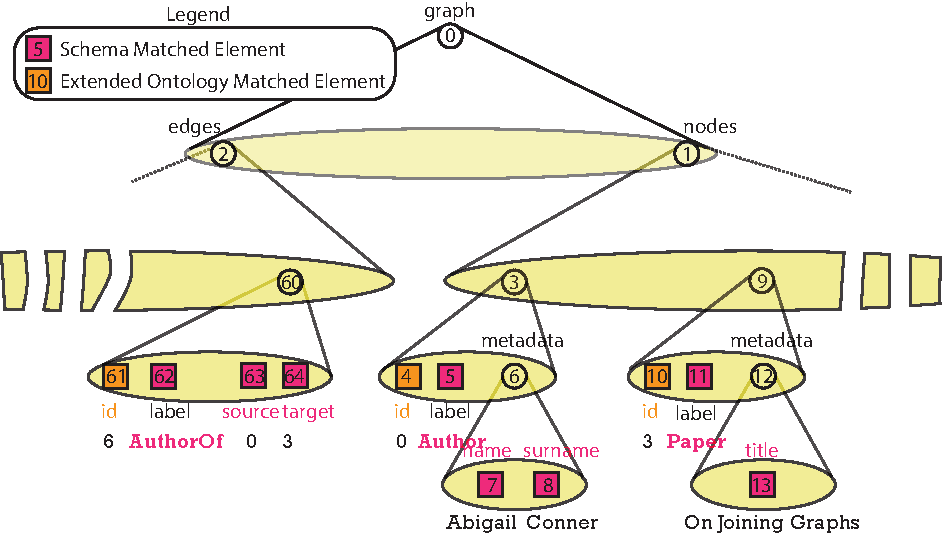
\includegraphics[width=\textwidth]{fig/04model/02MatchingKeyword}
		\subcaption{GSM representation of a subset of the $g$ JSON graph represented in Figure \vref{fig:jsongraphformat}.}
		\label{subfig:transformationandmatch}
	\end{minipage}
	\medskip
	
	\begin{minipage}{\textwidth}
		\centering
		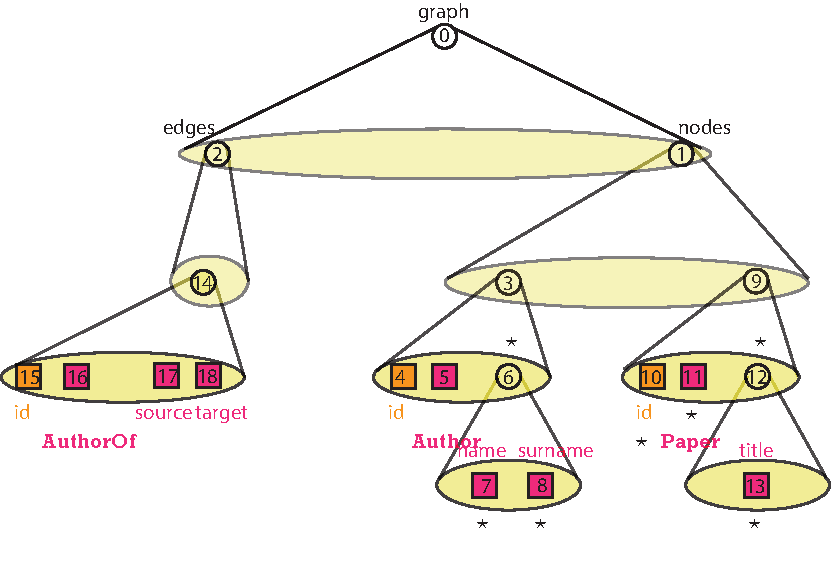
\includegraphics{fig/04model/03Schema}
		\subcaption{Schema extracted from the aggregation over the schema components found in the former GSM representation. Stars represent placeholders for the underlying data that has been ignore in the schema generation phase.}
		\label{subfig:jsonschemaextracted}
	\end{minipage}
	\caption{Manipulation of the JSON data for schema extraction.}
\end{figure}

Let us move on and discuss the relationship alignment phase. %In the following paragraph we'll show that the edge alignment process suffers from similar problems. 
The hub ontology already tells that an \texttt{Authorship} relation associates an \texttt{Author} (source) to a \texttt{Paper} (target). We now want to match such definition for the edges contained in the JSON representation $g$: even in this case an edge has a field called \texttt{source} and \texttt{target} as in the hub schema, but within our JSON representation \texttt{source} and \texttt{target} do not explicitly syntactically refer to a vertex, because \texttt{source} and \texttt{target} information is represented as a string (\texttt{Str}). Even if we stopped the analysis at this point, we would notice that it is impossible to draw scuh correspondences as an ``edge'' between the edge's source within the hub schema and any object represented in $\alpha(g)$. Even in this case, we must represent correspondences at a metalevel because no direct data manipulation is possible in practice.
%, as showed in the following paragraph.

Let us continue to draw correspondences at the meta level. Our data integration system already knows that \texttt{Author} and \texttt{Paper} in the hub schema are \ONTA(ies), and that \texttt{Authorship} is an edge connecting a vertex of the first type to a vertex of the latter. We can also freely assume that an internal dictionary will tell the system that \texttt{target} and \texttt{destination} are synonyms and that they both refer to \texttt{edges}. Similar considerations could be done for $\alpha(g)$, where only the \texttt{edges} field will be detected as containing a collection of edges. At this point, a word ontology such as Babelnet \cite{Navigli12} could tell that the term \texttt{Authorship} is related to the term \texttt{AuthorOf} used in $g$ representing an \texttt{edge}. Moreover, such JSON edges have a field called \texttt{source} and \texttt{target}, and hence there should be a correspondence between the JSON \texttt{AuthorOf} and the final graph \texttt{Authorship} edges, e.g. remarked by an $i$ variable:
\begin{lstlisting}[language=theoryjson,basicstyle=\ttfamily\small,mathescape=true]
graph.edges[$i$] : {source: Str, target: Str, label: Str, $\dots$}
graph.edges[$i$].label = "AuthorOf"
\end{lstlisting}
Moreover, with the previous alignment phase we also have found that \texttt{Author} and \texttt{Paper} are nodes, and then there should also be a correspondence between $source$ and $target$ as follows:
\begin{lstlisting}[language=theoryjson,basicstyle=\ttfamily\small,mathescape=true]
graph.nodes[$source$] : {label: Str, $\dots$}
graph.nodes[$source$].label = "Author"

graph.nodes[$target$] : {label: Str, $\dots$}
graph.nodes[$target$].label = "Paper"
\end{lstlisting}
In order to close the correspondence diagram, now we only have to detect which is the correspondence within the hierarchy associating each edge to a vertex: this could be done as previously through the extraction of associative rules, and hence we could determine that $source$ and $target$ within $g$ must refer to the nodes' $id$-s, thus allowing to extend the general edge rule as follows:
\begin{lstlisting}[language=theoryjson,basicstyle=\ttfamily\small,mathescape=true]
graph.edges[$i$] : {source: Str, target: Str, label: Str, $\dots$}
graph.edges[$i$].label = "AuthorOf"
graph.edges[$i$].source = $source$
graph.edges[$i$].target = $target$
\end{lstlisting}
We completed the alignment process via the enrichment of the hub schema through the extraction of associative rules. At this stage the alignment of $g$ with the hub schema is completed, and then we can use such correspondences to perform the sources' translation towards the hub schema representation. \qed
\end{example}
 

After describing how to carry out the data alignment within these two different data models (JSON and property graphs), we want to show how the previous data alignment process can be defined without any additional metalevel information by using GSM, which allows to represent both alignments and schemas. While in the previous example we needed to express further predicates and association rules in a distinct layer different from the data representation, in this incoming example such correspondences (morphisms)  are going to be expressed through an edge representation  as introduced in Definition \vref{sec:graphamatch}. If we want to create (hyper)edges having as targets the objects $o$ in the pattern $P$ and as sources one of the objects $\bigcup_{f_i\in m_P(\nested)}f_i(o)$ in $\nested$, such edges can be represented via the following object set:
\[w_{m,P,\nested}(o)=\Set{e_{oo'}|f_i\in m_P(\nested)\Rightarrow\phi(e_{oo'},\SRC)=f(o)\wedge \phi(e_{oo'},\DST)=[o]}\]
On the other hand, the function providing all the edges from the $\nested$ data source towards the matched object in $P$ is defined as follows:
\[\smatch_{m,P,\nested}(o')=\Set{e_{oo'}|f_i\in m_P(\nested), o'\in f_i(o)\Rightarrow\phi(e_{oo'},\SRC)=[o']\wedge \phi(e_{oo'},\DST)=[o]}\]
%Even in this case, we will leave for Chapter \ref{cha:nesting}  the way , %are stored. 
%while 
In the next example we are going to focus on how such data structures can support  correspondences' translation, while Chapter 7 will show how to instantiate and transform the matched parts after the definition of a query language over such data structures. Appendix \vref{appendix:realignments} provides the full source code describing  the following  example. 

\begin{example}[continues=ex:examplegraphdata,label=ex:examplereferencedOcaml]
We now must translate the hub schema into a nested graph representation as in Figure \vref{subfig:nestedhubforbiblio}. This other representation explicitly tells us that \RELA s have structural dependencies on \ONTA(ies), because each edge contains the information for the vertices. Hereby, the implication ``entities must be reconstructed before the edges'' comes for free from the traversal of the hub schema itself. Therefore, the schema alignment can be carried out by extracting the data's schema from the GSM-translated representation of the JSON objects: in particular, we can first perform a linear scan of the data (Figure \vref{subfig:transformationandmatch}) where the key elements of interest of the hub schema are selected (in magenta) alongside with other relevant terms (in orange). Then again, we aggreate each object in the data structure by the hub schema elements matched by each object, and hence we obtain the schema in Figure \ref{subfig:jsonschemaextracted}. Please note that the outline of the abstraction function $\alpha_1$	\index{$\alpha_1$} extracting the schema from the data acts similarly to the aggregation operator\footnote{This operation will be formalized as a derivate GSQL operator at page \pageref{abstractionAlpha1}. We can also think that the final id of the aggregated components depends on the list dovetailing $dtl$ of all the elements that have been aggregated, thus easing the subsequent transformation phase by reducing the visit time of the data data structure. }, and then new edge morphisms in $w_{\star,\alpha_1(g),g}$ are generated: in particular, $\star$ represents an arbitrary summarized value that can be induced by the aggregation $\alpha_1(g)$ of the input data ($g$); moreover, $\alpha_1(g)$ actually represents the schema for $g$ as required in the previous examples.  This means that GSM, as well as graphs semistructured data representations, allow to represent \textsc{Data} $g$ and \textsc{Model} $\alpha_1(g)$ at the same representation level.
% (see Definition \vref{sec:graphamatch}), thus providing correspondences between $g$ data objects and $\alpha_1(g)$ objects within the generated source schema:

%%even in this case, the usual property graph model does not allow do create edges where one of the 
%%%%1 
%%\hl{In order to carry out the alignments, we choose to translate the graph hub schema provided as an input into a nested graph representation depicted in Figure} . 
%
%%As a consequence, we must resolve the authors and the papers first, and then draw the edges. 
%
%
%%Also note that the correspondences between attributes of a given entity and the hub schema is now expressible within the generalized semistructured model thanks to its object representation and the definition of translation functions. 
%
%%At this point we can make one step further: even if a different attribute set can pertain to  
%
%% In order to do so,
%
%%At this point, we made a complete correspondence between the \texttt{authors} in source $g$ and the vertices in the final graph and, by the excluded middle law, we also characterized the \texttt{paper}. In all such cases the correspondencies could be expressed by equivalence relations.
%
%%As a last step for $g$, we want to extract the information concerning the edges (a.k.a. relationships): 
%%%2
%
%%We know that, within the hub schema, our final edges must satisfy the following pattern:
%%\[(source\colon\texttt{Author})\xrightarrow{\texttt{Authorship}}_i(target\colon\texttt{Paper})\]

%After this schema extraction phase, we can now suppose that each matched part within the original data is associated to the resulting    matching schema through \textit{morphisms} as outlined in Definition \vref{sec:graphamatch}, and used within Graph Grammars transformations (Definition \vref{def:graphgrammar}). In particular, shows that such morphisms may be represented as edges, where sources are the data elements and the targets are the schema elements expressed as a graph. 
After ``aligning'' the data object $g$ to the source schema ones $\alpha_1(g)$ obtained through aggregations of the objects in $g$, we want to continue with the (proper) schema alignment phase between the source schema and the elected hub schema: Figure \vref{subfig:match1} shows a traditional way to compare schemas, where correspondent entities are matched (even with this case) with an edge. Please also note that edges may be represented as nested graphs' edges and hence as objects even though, for representational ease, we distinguish such obects from the schema ones by representing them as arcs, similarly to what we did in the previous social network scenario. This schema matching representation must  distinguish\footnote{Such distinction, which is self-evident during the match creation phase, can be saved (e.g.) by storing the correspondences in different collections of a same object $\omega$; as an example $\phi(\omega,\mstr{ell})$ and $\phi(\omega,\mstr{xi})$ containments may collect these two types of correspondences.} the correspondences' edges in two main types: 
\begin{myalist}
\item orange dashed edges remark ``$\ell$''-matches that are objects containing similar (or identical) labels, and 
\item black uniform edges remark ``$\xi$''-matches establishing correspondences between %either objects having specific $\xi$ attributes or the hub schema's objects that are contained by another object via $\xi$, and 
objects $\tilde{o}$ in the source schema %with source schema objects exibiting such properties.
 and hub schema objects $\tilde{o}'$, appearing similar ``constrainable values''  according to a similarity predicate $\vartheta$; in particular the constrainable values are contained by either $\xi$ functions (e.g.,  $a\in\xi(\tilde{o})$ and $a'\in\xi(\tilde{o}')$) or the attribute through which the object is contained via $\phi$  (e.g., $a\in\Set{p| \exists o'.\tilde{o}\in \phi(o',p)}$ and $a'\in\Set{p'| \exists o'.\tilde{o}'\in \phi(o',p')}$).
\end{myalist}
%In particular, the ``$\ell$''-matches are used to check which are the elements referenced by the source schema that match the coarsest representation of an entity, while the ``$\xi$''-matches define either the constraints that have to be imposed over the entity-matched objects via $\ell$. We can distinguish two different possible types of such alignments: the ones that directly refer over the objects of interests, and the ones that are established through the containment attribute and, consequently, applied directly applied over the contained objects (and hence, falling on the first type). 
All the black arrows showed in Figure \vref{fig:alignmentrefinement} belong to such second scenarios, because the ``source'' and ``target'' values appearing in the source schema match with the containment attribute on the hub schema. Therefore, we can define the set of all the $\xi$-constrainable values appearing at a maximum\footnote{See line \ref{v3:cvBase} at Appendix A.} height $\delta$ from $o$ as follows:
\[cv_\delta(o)\eqdef\xi(o)\cup\Set{a|\exists o'. o\in\phi(o',a)}\cup\bigcup_{o'\in\varphi^\delta(o)}cv(o') \]
over which we can define our desired notion of object similarity over constrainable values\footnote{See line \ref{v3:cvTest} at Appendix A.} via a similarity predicate $\vartheta$:
\[cv_{\delta,\vartheta}(o,o')\Leftrightarrow \exists a\in cv_\delta(o).\exists a'\in cv_\delta(o').\vartheta(a,a')\]

While the ``$\ell$''-matches identify the possible translation of an entity in two different representations by comparing the \textsc{Model} pieces of information, the ``$\xi$''-matches identify the constraints that must be preserved in the transformation phase. Please also note that these considerations are valid if the data of choice represents the objects' types through $\ell$, and values or constraints through $\xi$-s.
\bigskip

%In particular, orange rectangles depict the matches between objects acting as attributes, purple elements remark the matching between source and target elements of the edge, and the red one remarks the alignment for the edges; green elements remark the matches obtained other the schema's labels; moreover, for each edge we shall store which component from the source and target object is object. As we can see, while 
We can now observe that such ``raw'' correspondences  can be refined by \marginpar{$\qedsymbol$ Alignment's refinement} transforming them with a $\ttransl$: while in the hub schema the \texttt{Author} node contains the attributes \texttt{name} and \texttt{surname}, in the data schema we have that the latter information is contained in a sibling object; therefore, the previous correspondences need to be post-processed to match each element of the hub schema with the coarsest representation within the data model. Therefore, we must reconcile each $\ell$-correspondence to the nearest $\xi$-correspondence, so that the reconciliation of the schema corresponding objects (happening on the next phase) will be eased. This $\ttransl$ process can be carried out with a depth postVisit\footnote{See line \ref{v3:postVisitPace} at Appendix A.} of the hub schema starting from its reference object, where the following operations are performed over the object $o$:

\begin{figure}[!t]
	\centering
	\begin{minipage}{\textwidth}
		\centering
		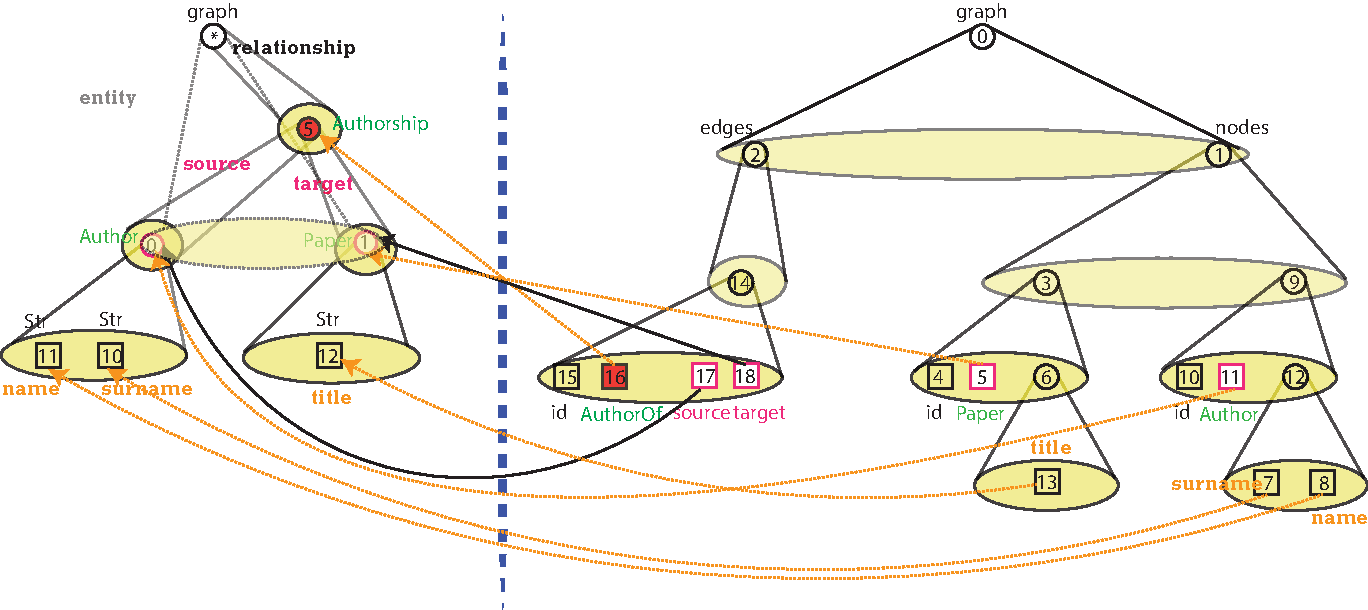
\includegraphics[width=\textwidth]{fig/04model/04aAlignment}
		\subcaption{Preliminar alignments (sketched as edges instead of objects in order to distinguish the two representations) based on either ontology or word similarity.}
		\label{subfig:match1}
	\end{minipage}
	\medskip
	
	\begin{minipage}{\textwidth}
		\centering
		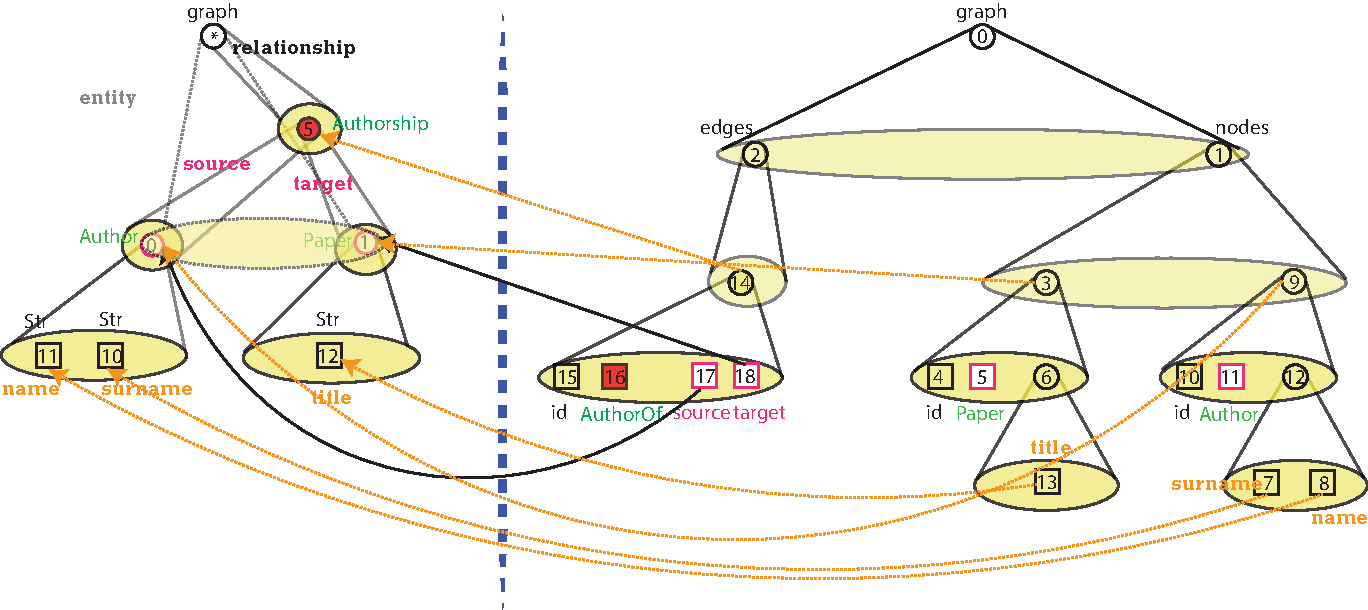
\includegraphics[width=\textwidth]{fig/04model/04bAlignment}
		\subcaption{Refactoring the previous alignments by comparing the depth of where such elements are located.}
		\label{subfig:match2}
	\end{minipage}
	\caption{Depicting two distinct phases of the entity alignments. Both the $\xi$  (dashed and in orange) and  $\ell$ alignments (in a black continuous line) are represented as object in order to visually distinguish them from the source (on the right) and hub  schema (on the left) objects.}
	\label{fig:alignmentrefinement}
\end{figure}
\begin{itemize}
	\item If the current element $o$ represents a leaf, no transformation occurs.
	%(i.e., an object with empty contents $\varphi(o)=\emptyset$), no operation on the correspondences is performed.
	\item Otherwise, after performng the preVisit\footnote{This means that $o$ is evaluated by the visiting algorithm before any other of its contents $\varphi(o)$.} on all the contents in $\varphi(o)$, update the  correspondences having $o$ as  a target, so that they are mapped to the $\alpha_1(g)$ coarset representation describing $o$ and $\varphi(o)$. This post condition is satisfied by the following procedure:
	\medskip
	
	Given $T$ the set of the $\ell$-matched having their targets $\{o\}\cup\phi(o)$ in the hub schema, let $S$ be the set of their sources in the source schema ($S\eqdef \bigcup_{t\in T}\phi(t,\mstr{src})$), we want to select the set of strongly nested object-set with respect to $\varphi^*(S)$, that is $\varphi^*(S)$ itself by definition. Now, we group all the correspondences in $T$ by their sources' membership to a specific element $a\in\varphi^*(S)$, that is:
	\[T_S\eqdef \Set{\Set{t\in T|a\in\phi(t,\mstr{src})}|a\in\varphi^*(S)}\]
	From each non empty collection $c\in T_S$, choose just one $\ell$-match $t_c\in c$ having a target object $o_{dst}^{t_c}$ (e.g., $o_{dst}^{t_c}\in\phi(t_c,\mstr{src})$) maximizing the absolute relative height $rh$ over $o'\in\{o\}\cup\varphi(o)$:
	\[t_c\eqdef \argmax_{\substack{t\in c,\\ t\in\phi(\omega,\mstr{ell})}}\Set{rh(o',\tilde{o})|\tilde{o}\in\phi(t,\mstr{dst}),o'\in\{o\}\cup\varphi(o)}\]
	Last, update $t_c$'s source to the common ancestor(s) of both $\ell$ and $\xi$ matches originating (i.e., having their sources) in $\phi(a_c)$, where  $a_c\in\phi(t_c,\mstr{src})$.

%	Given $T$ the set of the schema correspondences having their targets in $\{o\}\cup\varphi(o)$ (in the hub schema), let $S$ be the set of the correspondences' sources in the source schema ($S\eqdef \bigcup_{t\in T}\phi(t,\SRC)$) and let $\tilde{C}$ be the set of the strongly nested object-set  with respect to $\varphi^*(S)$, that is $\varphi^*(S)$ itself by definition. Now, group all the schema correspondences $T$ by their sources' membership to a specific element of $\varphi^*(S)$, that is:
%	\[T_{S}\eqdef\Set{\Set{t\in T|k\in c, k\in \phi(t,\SRC)}|c\in \varphi^*(S)S}\]
%	For each collection $c\in T_{S}$, choose the match $t_c\in c$ having $o$ as a target and that maximizes the absolute\footnote{By maximizing $|rh(o,o')|$ instead of $rh(o,o')$, we include the correspondence cases where the contents $\varphi(o)$ are aligned in $\alpha_1(g)$ as containers of $o$.} relative height $rh$ (Definition \vref{def:heights}) with the remaining elements in $c$:
%	\[t_c\eqdef\argmax_{\substack{t\in T\\ t\in\phi(\omega,\mstr{ell})}}\max\Set{\left|rh(o,\tilde{o})\right||o\in\phi(t,\SRC),\tilde{o}\in\phi^+(o)\cap c}\]
%	Last, update $t_c$'s source to the common ancestor(s) to all the elements in $\phi^*(a)\cap c$.
	
	%we group all the alignments having hub schema targets in $\{o\}\cup\varphi(o)$ by scl for each alignment we select all the schema alignments represented as edges $e_{oo'}$ of both the contents and container $o$ on the hub schema, having targets  by an arbitrary distance $\delta$, where the alignments' sources appear at a maximum distance of $\theta$ in the extracted schema. For each of those groups, we move the sources of the container's alignment towards the common ancestor of all the alignment's sources in the extracted schema.
\end{itemize}
Figure \ref{subfig:match2} depitcs the outcome of such process: while the matches over leaf objects subsume no refactoring, the others are refactored; for example, the \texttt{Author} element in the hub schema perfectly matches with the author representation within the \texttt{nodes} collections. Similar considerations can be carried out for the edges.

After consolidating the $\ell$-correspondences, we want to resolve both the morphisms and the alignment transformation by associating the data objects to the hub schema. Please note that the association of the results is only a preliminar step leading to the schema instantiation into some actual data. Such final process  { is going to be discussed in more detail in the next chapter with the help of GSQL, an ad hoc query language for GSM data representations}. 

At this point, we must ask ourselves how to traverse both schemas, \marginpar{Associating the data to the hub schema} hub and source, in order to associate the data objects to the final representation (similarly to the $Pop$\index{$Pop$!for $\Qoppa$} illustrated in Section \vref{subsec:dmalgebra}): this can be carried out by both traversing the schemas' alignment and the morphisms linking the data to its schema representation. This operation can be carried out using a postVisit \footnote{This means that, before visiting $o$, we postVisit the containts $o'\in\varphi(o)$, from the highest $o'$ to the lowest $o'$ w.r.t. $h_o(o')$, and then we evaluate $o'$ as a last step.} over the hub schema objects, starting from the reference object. 

For each currently visited object $\omega$, postVisit\footnote{See  line \vref{v3:performAssociations} at Appendix A.} the contained objects $\varphi(\omega)$ first; the contents are accessed by ordering them from the highest one with respect to the definition of $h_o$. For each visited object $o_i\in\varphi(\omega)$, the complete list of associations $\mathcal{I}_{o_i}$ is going to be returned\footnote{See line \vref{v3:postVisit} at Appendix A.}; each list $\mathcal{I}_{o_i}$ has an associated schema $\mathcal{S}_{o_i}$, which is a list of objects in the source schema to which $o_i$ corresponds via $\ell$-correspondences and subsequent refinements ($\mathcal{S}_{o_i}=\Set{\iota_{i_1},\dots,\iota_{i_m}}$); consequently, each element  $a\in \mathcal{I}_{o_i}$ is a list of lists $a=\Set{\lambda_{i_1}^a,\dots,\lambda_{i_m}^a }$ where $\lambda_{i_j}^a$ is a list of data objects corresponding to an object $\iota_{i_j}$ via the morphism\footnote{Refer to Definition \vref{sec:graphamatch} for this notion of morphism.} ${\iota_{i_j}}\to \lambda_{i_j}^a$. In order to use such $\lambda_{i_j}^a$ as constraints for the objects associated to our current object, we must first extract the set $\mathcal{I}_\omega$ of all the objects associated to it. This procedure\footnote{See line line \vref{v3:crossMorphisms} at Appendix A.} is defined as follows:
\medskip

	

{\narrower If \textbf{(i)} $\omega$ is a target for no $\ell$-correspondences, then $\mathcal{S}_\omega$ is the join of all the sources' schemas ($\mathcal{S}_\omega = \bowtie_{i\leq n} \mathcal{S}_{o_i}$) and $\mathcal{I}_\omega$ is the join between all the contents' associated values ($\mathcal{I}_\omega = \bowtie_{i\leq n}\mathcal{I}_{o_i}$). Otherwise, \textbf{(ii)}  $\mathcal{S}_\omega$ is the set $\Set{\jmath_{\omega_1},\dots,\jmath_{\omega_m}}$ of all the source schema objects $\jmath_{\omega_i}$ linked to $\omega$ via a $\ell$-correspondence $\jmath_{\omega_i}\to \omega$  and all the elements  $b\in \mathcal{I}_\omega$ are lists of lists $b=\Set{\lambda^b_{\omega_1},\dots,\lambda^b_{\omega_m}}$ where $\lambda^b_{\omega_i}$ is a set of data objects, which is associated to the source schema $\jmath_{\omega_i}$ via a morphism $\jmath_{\omega_i}\to \lambda^b_{\omega_i}$. This means that, in the second case, the data object referring to the parent $\omega$ are not (necessarily) restricted via the containment information. The only refinements may only occur via $\xi$ correspondences, as described in the following paragraph. \par}

{\narrower Next, if \textbf{(iii)} $\omega$ is a target for no $\xi$-correspondences, $\mathcal{I}_\omega$ is not restricted (or filtered). Otherwise, \textbf{(iv)} we must first create a set $\mathcal{I}_{\xi,\omega}$ for such correspondences, constructed similarly to $\mathcal{I}_\omega$ for the $\ell$-correspondences, and hence having an associated schema $\mathcal{S}_{\xi,\omega}$; then, for each $b\in \mathcal{I}_\omega$, we preserve each set $\lambda_{\omega_i}^b$ where there is at least one element satisfying one of the values associated to the objects in $e$, for each $e\in s$, where $s$ is contained in $\in\mathcal{I}_{\xi,\omega}$.\par}
\medskip

After defining $\mathcal{I}_\omega$, we can further skim the $\mathcal{I}_\omega$ using $\bowtie_{i\leq n}\mathcal{I}_{o_i}$ over $\mathcal{I}_\omega$, similarly to the steps outlined in \textbf{(iv)}\footnote{See line \vref{v3:crossLists} at Appendix A.}. After this further filtering, we can return $\mathcal{I}_\omega$ to all the possible containers, and hence terminate the postVisit for $\omega$. After terminating the postVisit for the reference object of the hub schema, we can use the instantiated hub schema and either return a graph by unnesting all the matched elements as it will be remarked for the $Pop$ operator presented at page \pageref{eq:popGraph} or even transform the content, as it will be showed in Section \vref{subsec:gggSec}. %Therefore, we will postpone the process of creation of new data from the matching in the next chapter.

%
%The data transformation phase finalizes the data integration steps that started through the establishment and update of alignments. %process.
%%The final alignment phase between edges is going to be carried out in the actual data transformation phase: in this scenario, 
%The hub schema will be now traversed using a postVisitrefining a set $\mathcal{I}$, containing the data objects that will correspond to the elements of the hub schema. Before starting such visit, $\mathcal{I}$ is initialized with all the objects from $g$; then, for each object $o$ of the hub schema appearing in the postVisit, $\mathcal{I}$ is restricted and then passed to all the components $\varphi(o)$. %d  of the aligned objects of the original data from which the schema has been extracted: at each visiting step %the set $\mathcal{I}$ of the possible objects over which apply the instantiations of the hub schema will be defined by the object set obtained at the container level; each containing object 
%The restrictions are derived from the evaluation of the $\lambda$- and $\xi$-matches over $g$ via the morphisms mapping $\alpha_1(g)$ to $g$: \textbf{(i)} if for the current object $o$ ``$\lambda$''-matchings $l\in L$ exist, we restrict $\mathcal{I}$ to the data objects associated to $\alpha_1(g)$ objects $\lambda$-matched in $L$, that is:
%\[\mathcal{I}=\mathcal{I}\cap \bigcup_{l\in L}w_{\star,\alpha_1(g),g}(\phi(l,\SRC)[0])\]
%%a new vertex is visited, which will apply some restrictions over $\mathcal{I}$, and then will provide such restricted object set to all the contained components. In particular, the root will initialize $\mathcal{I}$ with all the possible objects of the data set. At each preVisited step, 
%Then, \textbf{(ii)} we must group all the object in our updated $\mathcal{I}$ according to the similar values referenced by the ``$\xi$''-matches over $o$ according to the $cv_\vartheta$ similarity as follows:
%\[\mathcal{I}_\vartheta \eqdef\Set{\Set{j\in w_{\star,\alpha_1(g),g}(\phi(e,\SRC)[0])| cv_\vartheta(i,j)}|i\in \mathcal{I}}\]
%%we must analyse both aforementioned kinds of alignments. If for the current objects there exists ``$\lambda$''-matchings, we restrict $\mathcal{I}$ to such data objects (and their contents) having morphism mapping to schema objects which are already sources of $\lambda$-matches arriving at the current hub schema object\footnote{In such way we restrict the object of interest to the one that comply with both schemas.}. At this point, we must group all such $\mathcal{I}$ values according to the ``$\xi$''-matchings $e_1,\dots e_n$ having the current object or its contents in $\varphi(o)$ as a target; each group will be formed by the data objects, which are mapped to schema elements appearing as sources of $e_1,\dots,e_n$: for each $e_1,\dots,e_n$, we map them to their source objects $s_1,\dots,s_n$ in the schema, where each $s_i$ is associate to a set of morphisms $\Set{f_{s_i^1},\dots,f_{s_i^{m_i}}}$ which length $m_i$. The, we want to select one morphism $f_{s_i}^{j_i}$ for each source $s_i$, so that we create a group of morphisms\footnote{This part outlines the scenario where I have multiple constraints coming from multiple sources: e.g., } $f_{s_1^{j_1}},\dots,f_{s_n^{j_n}}$, where each subgroup of data objects mapped through morphisms and ``$\xi$''-alignments to one single hub schema object having the similar set of $\xi$ values. Such value similarity may be expressed through an $n$-ary similarity predicate $\theta$, possibly an $n$-element equivalence. The data objects referenced by $f_{s_1^{i_1}},\dots,f_{s_n^{i_n}}$ will be part of one possible restriction of $\mathcal{I}$, as well as the data objects $\tilde{o}$ and their contents $\varphi(\tilde{o})$, having an association with a schema object $\overset{\approx}{o}$ via morphisms and where $\overset{\approx}{o}$ is a source for a ``$\lambda$''-match sharing the target with one of the $e_1,\dots,e_n$. By doing so we check that all the schema values constraints through ``$\xi$''-matchings are satisfied, and we also make sure that such matches represent components for new entities involved in a ``$\lambda$''-matching phase. Over these objects, we can possibly apply a transformation which is associated through a $\xi$ expression represented in the hub schema. 
%For each of such restrictions of $\mathcal{I}_\vartheta$ we will continue to postVisit the hub schema objects contained in $\varphi(o)$ from the initial object $o$: in particular, we will continue the visit by sorting the contents of $\varphi(o)$ (if any) from the ``highest'' non-visited child to the ``lowest'' non-vistited one, according to  $h_{o}(o'')$ provided in Definition \vref{def:heights}.
%
%{\color{red} TODO: la postvisita, dopo che ho ottenuto tutti i sottogruppi restituiti dall'elemento padre.}


  %object, we must distinguish the different kinds of alignments: the alignments that have been done over the $\xi$ properties of an object, regard the constraints defined within the hub schema, while the ones performed over the $\lambda$ elements regard the entity and relationship matching, from which we can extract the values that we will then instantiate on the schema. From all the $\xi$ alignments, we must group them by selecting the ones sharing the same set of informations $\iota$ ($\xi$ or $\lambda$) in the objects that was grouped to obtain the correspondent object in the schema. For each of these groups, we select the $\lambda$ alignments where all the sources $s$ contain, at any nesting depth, the $\iota$ values. For each of these $s$ sets, we restrict $\mathcal{I}$ to $s$, instantiate the values required by the schema as a result of the matching, and continue the visit to all the subset. 

Please observe that the alignment of $g'$ with the hub schema could be carried out similarly, except for the process requiring to align \texttt{fullname} with both \texttt{name} and \texttt{surname}. If both $g$ and $g'$ share a common subset of data sources, then we could try to perform a match between all the values associated to the attirbutes defining an \texttt{Author} \cite{Jagadish}. Since in $\alpha(v')$ there is just one field for the \texttt{Authors}, \texttt{fullname}, while in $\alpha(g)$ we have both \texttt{name} and \texttt{surname}, we could  try to find some correspondencies and manage to find that \texttt{fullname} is just a combination of \texttt{name} and \texttt{surname}. When such task is not generally possible because the two bibliographic network belong to different conferences with authors with different research interests, then the only way to associate \texttt{fullname} with \texttt{name} and \texttt{surname} is to use an ad-hoc ontology containing informations regarding such ontology, thus allowing to perform the whole alignment process.
\end{example}

This last example showed us that the whole alignment  process of the hub schema towards the dataset via the dataset's schema resembles an approximated alignment. In particular such matches are refined through a $\ttransl$ translation  based on the data content  through the correspondencies.% and then rewritten using the hub schema. %Consequently, such process resembles the refinement and matching  graph grammars, where the graph alignment and rewriting graphs correspond to the same hub schema. %Therefore, a generalization of graph grammars is going to be provided (Section \vref{subsec:gggSec}). 
%In particular, the previous example outline one of the possible ways to perform graph alignment, after which instantiate the schema. This process will allow to create a new nested graph which schema corresponds to the hub schema.
After this preprocessing and data association phase, we can manipulate the matched data by associating it to the hub schema through $\varphi$ containment relations. In the thext chapter we are going to see a different approach for data integration, where the data matched by traversing the morphisms may be also transformed into new object not pre-existing the data source.